\chapter{Introduction}
\label{chap:introduction}

In an article published in 2002, Matt Ward stated that data sizes were exploding \cite{ward02}.
Since then, the rate of data growth has not relented.
Facebook, Twitter, LinkedIn, and Google Plus, all of which did not exist in 2002, contribute huge amounts of information to government departments, marketers, and social scientists.
The democratisation of DNA sequencing technology combined with a scientific need to bring together many different data sources in to their analyses (\eg, RNA, proteomic, metabolomic, and clinical chemistry data) has pushed the biological sciences into a more data-centric domain.
Since 2008, physicists can now get their hands and algorithms on over 20 petabytes of information every year from the large hadron collider at CERN.
By bringing together lots of information from different sources, it is commonplace for a data record to have anything from tens to thousands of quantitative and qualitative data variables (termed multivariate data) \cite{ward02}.

So how does one deal with such data and interpret it?
Statistical techniques are effective in the detection of trends and outliers in data where there is a pre-existing model of what is expected.
However, they are not so effective in the detection of trends and outliers in data when no such model exists.
The human perceptual system is incredibly powerful at finding patterns or outliers that statistical techniques may miss.
When no model is yet known or unavailable, or when uncertainty exists on an underlying model, visualization can take advantage of the human perceptual system to help users in a number of tasks, including:
\begin{enumerate}
\item observation of trends and outliers;
\item creating connections between data and past experience, knowledge, and intuition;
\item visual generation and evaluation of hypotheses;
\item monitoring the correctness and performance of computational models; and 
\item effective communication with others.
\end{enumerate}

\begin{figure}[t!]
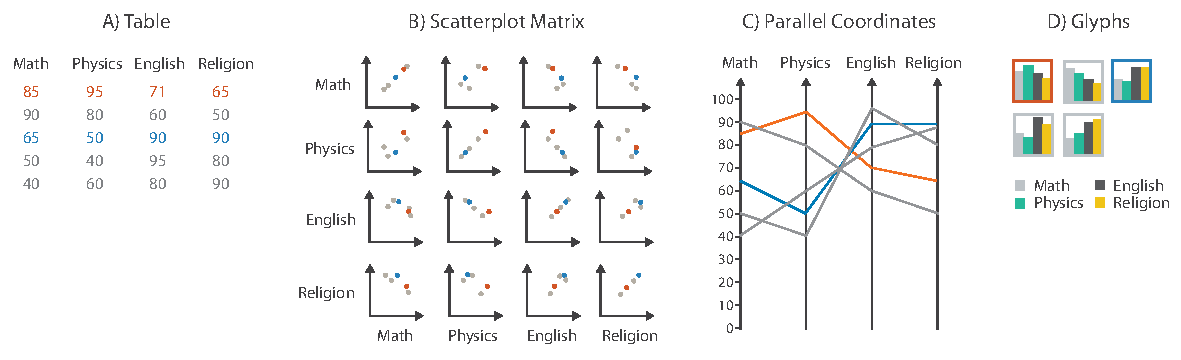
\includegraphics[width=\textwidth]{images/introduction/multivariate_vis}
\caption{Techniques for multivariate data exploration include: A) tables; B) scatter plot matrices (SPLOMS); C) parallel coordinate plots; and D) glyph-based visualization.}
\label{fig:multivariate_vis}
\end{figure}

Multivariate data visualization is a class of visualization techniques that deal with the presentation of many data record attributes at once.
Four primary multivariate data visualization techniques displayed in Figure \ref{fig:multivariate_vis} are:

\begin{enumerate}
\item \textbf{Data Tables} (Figure \ref{fig:multivariate_vis} A) are the simplest and most pervasive form of visualization.
There are many limitations to tables over more graphical visualization techniques generally around scalability (you can only view a limited number of rows at a time), and trend/outlier identification problems (it is hard to see large scale trends in a table);

\item \textbf{Scatter plot matrices (SPLOMS)} (Figure \ref{fig:multivariate_vis} B) where each dimension of a record is plotted against other dimensions \cite{Elmqvist2008Scatter} as an individual scatter plot.
This technique suffers in that $N^2$ plots are required where $N$ is the number of dimensions.
So while this technique is effective for a small number of dimensions, its capabilities diminish as the number of dimensions grow; 

\item \textbf{Parallel coordinate plots} (Figure \ref{fig:multivariate_vis} C) encode each variable/dimension of a data record as an axis with a line passing through each axis at the point given by the data record.
A full review of parallel coordinates can be found in a STAR from Heinrich and Weiskopf \cite{heinrich2012state}; and

\item \textbf{Glyph-based visualization} (Figure \ref{fig:multivariate_vis} D) uses visual items (termed glyphs) to encode data attributes using a number of visual channels (\eg, colour, shape, size, position, etc.).
These glyphs can then be positioned independently in 2D or 3D space to form the overall visualization.
\end{enumerate}


\section{Glyph-based Visualization Challenges}
While tables, SPLOMs and parallel coordinate plots can be deployed relatively easily, \emph{effective} glyph-based solutions are generally more difficult to implement.
Glyph-based visualization is a powerful technique, offering an advantage over other multivariate data visualization techniques in their ability to preserve spatial information.
However, their implementation is not straightforward and a number of challenges exist within information visualization (largely 2D) and scientific visualization (largely 3D).
Drawing from the State of the Art Report (STAR) on glyph-based visualization from Borgo \etal \cite{Borgo:2013:EG}, and Matt Ward's paper on ``Multivariate Data Glyphs: Principles and Practice'', the following challenges can be extrapolated:


\begin{enumerate}
\item \textbf{Technical Challenges}:
	\begin{enumerate}
		\item \textbf{Challenge 1} - \emph{Glyph Placement} concerns how glyphs are arranged spatially in 2D or 3D scenes.
		Position is an important visual channel, therefore ensuring glyphs are displayed in the right position is a key problem in many domains.
		
		Matt Ward's excellent survey on glyph placement provides a great overview of a number of strategies for glyph placement that includes data- and structure-driven techniques \cite{ward02}.
		Ropinski \cite{ropinski11} added a further strategy for medical data, named feature-driven glyph placement which places glyphs on particular features of the underlying data.
		Borgo \etal \cite{Borgo:2013:EG} also added user-driven glyph placement as a categorisation.
		Glyph placement remains a problem within the visualization community due to problems with occlusion for example.
		
		\item \textbf{Challenge 2} - \emph{Data Ordering} considers how data records can be ordered or have sets of variables grouped to highlight specific trends or interesting parts of the data\cite{ward08}.
		The ordering of the underlying data can influence how particular features of the data are interpreted during analysis and is very much task dependent.
		For example, if a user is using a glyph-based visualization to gain an overview of how much customers have spent over the past year, having randomly ordered monthly totals is not going to be as useful as having the months arranged naturally from January to December.
		
		\item \textbf{Challenge 3} - \emph{Glyph-based Visual Compression} is a technique that uses glyphs to reduce the amount of visual space taken up in a display by common patterns/motifs.
		A key challenge in this technique is determining which parts of the data are not only common, but will also visually compress the most space.
		Additionally, instead of ad-hoc compressions of data, a further challenge would be in creating glyph libraries to be used across a domain to consistently represent common features in their data.
		
	\end{enumerate}
\item \textbf{Design Challenges}:
	\begin{enumerate}
			\item \textbf{Challenge 4} -  \emph{Data to Visual Mapping} relates to how particular data variables are mapped to colour, shape, size, and texture for example (called visual channels).
			Mappings can vary depending on the type of the data variable (\eg, categorical or quantitative) with not all visual channels being equally good or bad at representing either type of variable.
			Challenges exist in determining which data items should be represented by which visual channels.
			For example, some visual channels are perceived together (integrally) rather than separately.
			The result is two data variables being mapped to integral visual channels, thereby hiding aspects of the original data record.
			Additionally, colour is a powerful visual channel, while texture is not.
			How can a glyph designer decide over whether to use colour for one variable, and texture for the other?
			
			\item \textbf{Challenge 5} - \emph{Glyph Arrangement} refers to how a glyph will arrange its constituent parts.
			This is often required for more complex glyphs that are representing many dimensions.
			For example, in Chernoff faces various data values are mapped to facial features such as face, nose, and eye dimensions.
			In this case, the arrangement of glyph features is given due to the natural ordering of facial features, but this is not always the case.
			
			This relates to glyph distinguishability which is concerned with how glyphs are perceived at different resolutions.
			By ensuring that variables important to the user tasks are available when glyphs are small, users will be able to use many glyphs on a screen at once, and visually filter for glyphs representing data items of interest.
			
			A key challenge for glyph arrangement is in the provision of more systematic methods for deciding how visual channels can be composed to form a glyph.
			
	\end{enumerate}
	
\item \textbf{Evaluation Challenge}:
\begin{enumerate}
	\item \textbf{Challenge 6} - \emph{Quality Measurement}. Numerous examples of glyph-based visualization are applied to the medical domain.
	In such domains, obtaining enough attention from a domain expert (a doctor or consultant) in order to carry out a meaningful evaluation is difficult.
	It is therefore hard to fully evaluate glyph \emph{memorability}, \emph{distinguishability}, \emph{interpretability}, and \emph{utility} of a glyph set.
	Therefore a key challenge is in finding ways other than through user interaction, to assess typical evaluation metrics.
\end{enumerate}

\end{enumerate}

In this thesis, we investigate a number of these technical, design, and evaluation challenges of glyph-based visualizations through the provision of a more systematic process towards glyph design .
This systematic process largely involves the heavy use of computational techniques (accompanied by design principles) to investigate the following three questions:

\begin{enumerate}
\item \textbf{Is glyph design amenable to systematization by computational methods?}
How can one go from data values to a visual channel, and how can these channels be organised in to a coherent glyph?
Well-designed glyphs can greatly enhance visual search and pattern identification, and are intuitive to learn and use.
However, as Ward stated, the selection of one visual channel over another could have direct implications on how an attribute is perceived and interpreted by an observer \cite{ward02}.
For example, some visual channels are better at representing qualitative information while others are better at representing quantitative information.
Additionally, glyphs are often small, therefore visual channels will have relatively limited bandwidth capacities.
How can a glyph be designed to ensure that important information is visually accessible to users?

This question investigates \textbf{Challenges 2, 4, and 5} from the glyph challenges stated above.


\item \textbf{Can computational methods be applied to the design of glyph libraries for visual compression?}
A further application area for glyphs is in the visual compression of information.
Most displays will have a screen width of approximately two thousand pixels.
This means that for time series data for example, you can plot two thousand values (considering no need for connecting lines) before having to sample the data.
If common patterns in the data (motifs) were represented as a glyph library, the data could be compressed, leaving the ``interesting'' parts of the data in a more digestible form for users.
The question is, how can such a glyph library be designed?
In some domains, common patterns may be known by domain-experts, and this could form the basis of the glyph library.
In other domains, the library will evolve as a result of many years of refinement.
In other domains however, little may be known, so how can decisions be made on which data should be represented by glyphs?
Can computation play a role in controlling this process?

This question investigates \textbf{Challenge 3} from the glyph challenges stated above.

\item \textbf{Are there areas of evaluation that can be performed more systematically?}
Evaluation is normally carried out by human observers in time-consuming studies.
The results and impact of such studies can be limited by the number of domain experts.
We wish to investigate how evaluation can be made more systematic and whether computation can replace humans in some aspects of glyph evaluation.

This question investigates \textbf{Challenge 6} from the glyph challenges stated above.

\end{enumerate}

\section{Thesis Scope}
The scope of this thesis falls within the greater subject area of Computer Science, specifically \emph{Computer Science} $\rightarrow$ \emph{Visual computing} $\rightarrow$ \emph{Visualization} $\rightarrow$ \emph{Information visualization} and \emph{Visual analytics} $\rightarrow$ \emph{Glyph-based, high-dimensional visualization}.


Visualization as a domain is spanned across two major areas.
These areas, defined by the freedom to choose where elements are spatially positioned in a visualization are as follows:

\begin{enumerate}
	\item \textbf{Scientific Visualisation (SciVis)} is built upon the underlying premise that spatial position is \emph{given} within the data set \cite{munzner2014visualization, telea2014data}.
	This means that visualization designers do not have a choice in where to position elements.
	The majority of \emph{SciVis} contributions are therefore spatial data visualizations.
	
	\item \textbf{Information Visualisation (InfoVis)} concerns visualization challenges where the use of space is \emph{chosen} by the visualization designer \cite{munzner2014visualization}.
	Due to the choices involved, and the subjectivity often present in making these choices, the domain of \emph{InfoVis} is largely concerned with determining whether of not the chosen design is fit for purpose, hence the design studies and evaluations that populate the \emph{InfoVis} category.  
\end{enumerate}

Additionally, Visual analytics (extensively featured in the Visual Analytics Science and Technology (VAST) Conference at IEEE VIS) is a relatively new field that spans the \emph{scientific} and \emph{information visualization} domains.
Visual analytics is often defined as the``integration of analysis, visualization and interaction".
The benefit of this paradigm is that visual analytics brings together the processing capabilities of computers and the pattern recognition, and hypothesis generating capabilities of humans.


Furthermore, additional research venues are appearing that encompass domain-specific groupings of visualizations that are somewhat free of the \emph{SciVis}, \emph{InfoVis}, and \emph{VAST} categorisations.
For example, in biology there is BioVis (\url{http://www.biovis.net/}), and for security there is VisSec (\url{http://www.vizsec.org/}).

The work presented in this thesis has solely focuses on \emph{information visualization} and \emph{visual analytics} with application areas in biology and security.

\section{Thesis Organization and Contributions}
The thesis from hereon in is organised into seven chapters that collectively aim to answer the above questions. 

\textbf{Chapter \ref{chap:related_work}} provides a detailed view of the psychology literature describing the various properties of the human visual system and how this can be exploited in glyph design.
We follow with an overview of the large body of research in glyphs from their origins to their present day use.
The latter part of this chapter is based upon a STAR report co-authored with Borgo \etal \cite{Borgo:2013:EG}. 

\textbf{Chapter \ref{chap:strategies}} proposes a model representing a more systematic glyph design process.
This model will be applied throughout the thesis to determine its applicability to a number of glyph-based visualization challenges.

\textbf{Chapter \ref{chap:glyph-tax}} details a systematic way of creating glyphs using a taxonomy-based approach for the replacement of text labels in biological workflows. 
This work addresses a number of technical and design glyph-based visualization challenges.
First we provide a novel solution to a technical challenge through algorithmic creation of a taxonomic tree for \emph{Challenge 2 - Data Ordering}.
This involved the creation of a novel algorithm for the classification of a large corpus of qualitative data to create a balanced tree.

We then proceed to address two design challenges.
Visual channels are ordered by their strength and a number of perceptual guidelines are highlighted which relates to \emph{Challenge 4 - Data to Visual Mapping}.
This ordering is based on a large review of the psychology literature on human perception from Chapter \ref{chap:related_work}.

Finally, we propose a solution to \emph{Challenge 5 - Glyph Arrangement} by using the taxonomic tree to guide the creation of glyphs.
The top level of the tree is represented by the strongest visual channels, and the lowest levels of the tree are represented by the least prominent visual channels.
We propose a test for the final glyph arrangement via a ``crush'' test that can be used to determine whether or not the important information in the glyph is available to observers even at low resolutions.


This work was published in IEEE TVCG in a publication by Maguire \etal \cite{Maguire:2012:TVCG} and presented in the InfoVis track at IEEE VIS 2012.
Additionally, the basis of this work forms a key component of the IEEE VIS 2014 tutorial on glyph-based visualization\footnote{\url{http://ovii.github.io/IEEEVisGlyphTutorial/}}. 
This work was jointly performed with Philippe Rocca-Serra, Susanna-Assunta Sansone, Jim Davies and Min Chen.  
The implementation and paper writing was conducted by Eamonn Maguire, Min Chen guided the work, and Philippe Rocca-Serra, Susanna-Assunta Sansone, and Jim Davies provided further domain knowledge and validated the technique.\\

\textbf{Chapters \ref{chap:automacron}} and \textbf{\ref{chap:timeseries}} investigate how computation can help in the design of glyph libraries for visual compression.
Both chapters investigate a technical glyph-based challenge in \emph{Challenge 3 - Glyph-based Visual Compression} for two data types, graph and time series data respectively.\\

\textbf{Chapter \ref{chap:automacron}} investigates the compression of workflow visualizations introduced in Chapter \ref{chap:glyph-tax} with automatically created glyphs.
This involves the creation of a novel frequent pattern (motif) finding algorithm for directed acyclic graphs.
This algorithm advances on previous algorithms through the ability to discriminate between types of nodes and edges in motifs.
By running the algorithm over 10,000 workflows, we can determine the common motifs.
Glyphs are automatically created for the most common motifs to form a library of `macro' glyphs, similar in concept to macros used in electronic circuit diagrams for example.
The resulting glyph library is used to visually compress biological workflows. 

This work was published in IEEE TVCG in a publication by Maguire \etal \cite{maguire13} and presented in the InfoVis track at IEEE VIS 2013.
The work was jointly performed with Philippe Rocca-Serra, Susanna-Assunta Sansone, Jim Davies and Min Chen.  
Implementation, and paper writing was conducted by Eamonn Maguire, Min Chen guided the work, Philippe Rocca-Serra, Susanna-Assunta Sansone, and Jim Davies provided domain knowledge to validate the technique.\\

\textbf{Chapter \ref{chap:timeseries}} builds on the research presented in Chapters \ref{chap:glyph-tax} and \ref{chap:automacron} with the use of glyphs for the visual compression of time series data.
We present a novel algorithm to find frequent long patterns (FLPs) or motifs in a corpus of time series data. 
This algorithm can be refined using a visual analytics platform required due to the parameter tuning required for different data domains.
Resulting motifs are automatically represented by glyphs, and these are used to visually compress a time series, leaving anomalous regions in place.
The work was jointly performed with Susanna-Assunta Sansone, and Min Chen.
Implementation was conducted by Eamonn Maguire, Susanna-Assunta Sansone helped in presenting some biological use cases, and Min Chen guided the work.\\

\textbf{Chapter \ref{chap:processes}} presents a number of glyph design processes and evaluation methods in addition to those used in the Chapters \ref{chap:glyph-tax} to \ref{chap:timeseries}. These processes and evaluations have been applied to three diverse cases: 
\begin{enumerate}

\item \textbf{Biological sequence visualization (DNA, RNA, and amino acid)} which focuses on the improvement of an existing design for visualization of biological sequence ``logos'' that show areas of DNA/amino acid conservation across different species.
We create a new glyph to represent conservation at each position in a sequence, and add additional glyphs to help users interpret why these changes happen.

This work investigated how much of the perception research gathered throughout the thesis could be used to improve a visualization.
This relates to challenges \emph{Challenge 4 - Data to Visual Mapping} and \emph{Challenge 5 - Glyph Arrangement}.
We investigated how the existing ``sequence logo'' visualization could be improved to improve data interpretation by considering research presented in Chapter \ref{chap:related_work}, especially that relating to spatial frequencies and global/local processing.
Additionally, by ordering the arrangement of elements within the glyph, we aimed to further improve the interpretation of our results.
An online evaluation encompassing over forty bioinformaticians and biologists confirmed that our approach had improved interpretation.

The work was published as a short paper and presented at EuroVis 2014 in a paper entitled \emph{Redesigning the Sequence Logo with Glyph-based Approaches to Aid Interpretation} \cite{CGF:maguire14-sp}.
The design, implementation, and paper writing were performed by Eamonn Maguire.
Design options discussed with Susanna-Assunta Sansone, Philippe Rocca-Serra, and Min Chen;

\item \textbf{Poetry visualization} where we present two pieces of work focusing on glyph-based solutions for poem visualization.
The first focuses on the design of a representation for twenty-six poem variables. 
This work was performed with: Alfie Abdul-Rahman who performed requirements elicitation, implemented the software, and conducted evaluations; Min Chen who led the project; numerous researchers from Oxford and Utah who participated in the requirements gathering and evaluation processes; and Eamonn Maguire who designed the poem glyphs.

This work presents a solution to \emph{Challenge 4 - Data to Visual Mapping} through the provision of a user-driven approach to data mappings between data and their respective visual encoding.
The rule-based approach applied to this mapping process provides some assurances over the quality of mappings, by ensuring users do not choose unsuitable mappings or overload the use of particular visual channels.

This work was published in the Computer Graphics Forum in 2013 in a publication by Abdul-Rahman \etal named \emph{Rule-based Visual Mappings -- with a Case Study on Poetry Visualization} \cite{CGF:Abd2013a}.
 
The second focuses on the design of a ``macro'' glyph to show the changes in the sounds of each line of a poem.
This work presents a solution to \emph{Challenge 5 - Glyph Arrangement} through the use of statistical data analyses to inform the ``macro'' glyph design.

This work was performed with: Alfie Abdul-Rahman who performed requirements elicitation, participated in the glyph design process through performing a statistical analysis of the data, and conducted evaluations; Min Chen who led the project; and Eamonn Maguire who worked on the glyph design and implementation processes.
It was published as a short paper in 2014 in a publication by Abdul-Rahman \etal named \emph{Comparing Three Designs of Macro-Glyphs for Poetry Visualization} \cite{CGF:abdul-rahman14-sp}; and

\item \textbf{File system visualization} which involves the application of glyph-based techniques to the visualization of file system events. 
We present an approach for the creation of visually separable glyphs using a metric based on the minimal Hamming distance.
With this, we propose a computational technique for conducting evaluations on glyph distinguishability.

This work presents a partial solution to \emph{Challenge 6 - Quality Measurement} through the use of computation as a way of evaluating glyph distinguishability.

This work was jointly performed with Phil Legg, Simon Walton, and Min Chen.
Implementation was conducted by Eamonn Maguire and Simon Walton, Phil Legg oversaw the evaluation, and Min Chen guided the work.
A manuscript is in preparation that was contributed to by all five researchers.
\end{enumerate}

Finally, \textbf{Chapter \ref{chap:conclusion}} brings a close to the thesis with a discussion on its contributions and future research directions triggered from this work.
